\chapter{Spark}

\section{Job description}

A unique Spark file will execute all jobs specified in section \ref{workflow}. The dataset is loaded as a Spark ``DataFrame'' and every operation will lean on ``SparkSQL'' layer.

Figure \ref{fig:spark-DAG} shows the complete DAG correspnding to the main job created by Spark. Figure \ref{fig:spark-DAG-info} shows Spark DAG accompained with few extra info.

\begin{figure}[H]
	\centering
	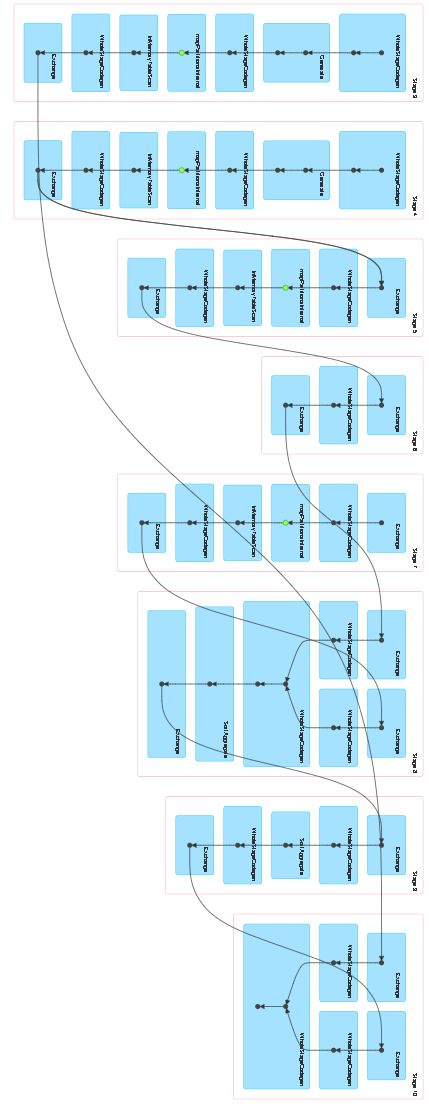
\includegraphics[scale=0.8]{images/3-spark/spark-DAG.png}
	\caption{Complete Spark DAG.}
	\label{fig:spark-DAG}
\end{figure}

\begin{figure}[H]
	\centering
	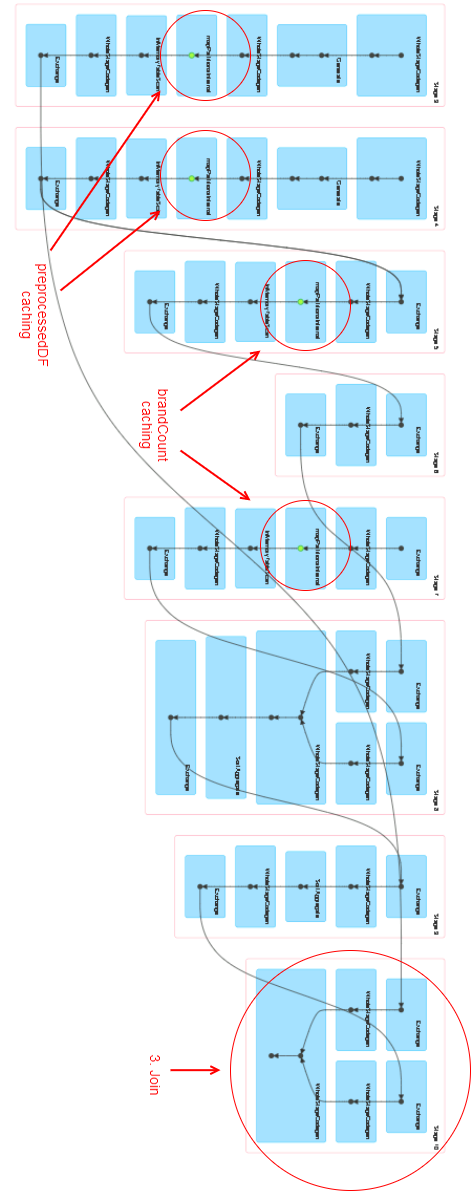
\includegraphics[scale=0.8]{images/3-spark/spark-DAG-info.png}
	\caption{Extra info about Spark DAG.}
	\label{fig:spark-DAG-info}
\end{figure}

Since the size of tables used in the two join operations is not excessive, the usage of the broadcast feature may be used on one table. Such an operation makes Spark split the job in three pipelined different jobs (few stages are skipped though).

The broadcast version results on an overall of 800 tasks (against the 1200 of the basic one), a more efficient usage of memory (garbage collection time) and a decrease of execution time close to 8/9\%.

DAGs for the broadcast version are reported in figures \ref{fig:sspark-broad-DAG-1}, \ref{fig:spark-broad-DAG-2} and \ref{fig:spark-broad-DAG-3}.

\begin{figure}[H]
	\centering
	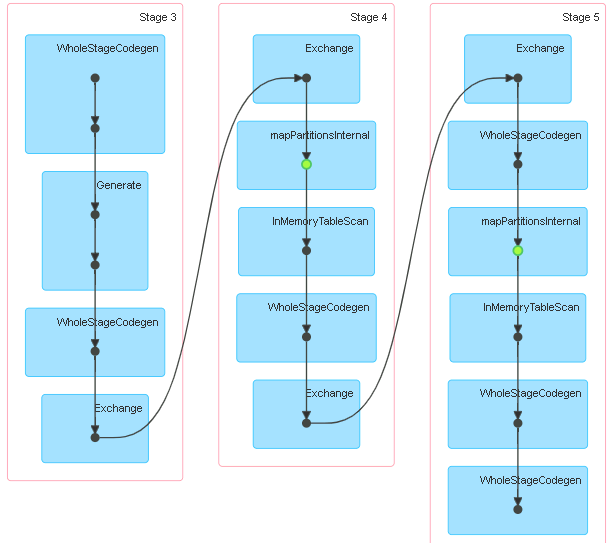
\includegraphics[scale=0.8]{images/3-spark/broad-DAG-1.png}
	\caption{DAG for first job created by Spark when using broadcast on join.}
	\label{fig:sspark-broad-DAG-1}
\end{figure}


\begin{figure}[H]
	\centering
	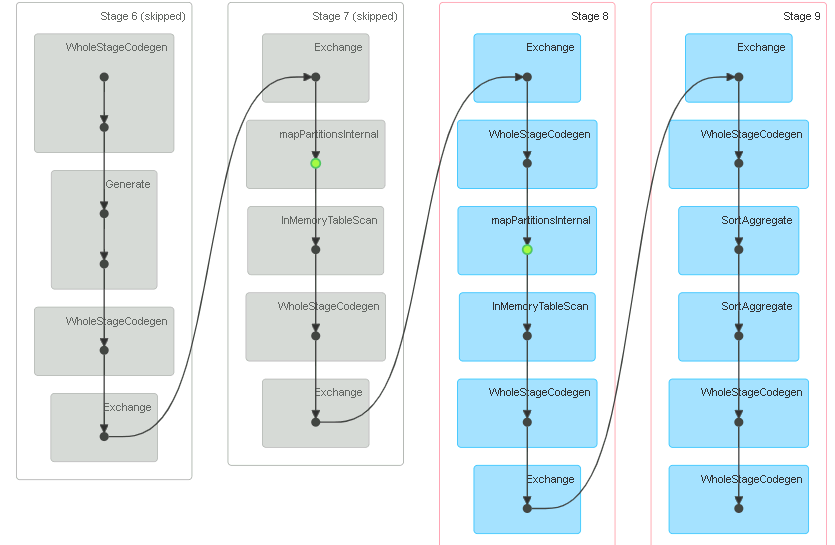
\includegraphics[scale=0.65]{images/3-spark/broad-DAG-2.png}
	\caption{DAG for second job created by Spark when using broadcast on join.}
	\label{fig:spark-broad-DAG-2}
\end{figure}


\begin{figure}[H]
	\centering
	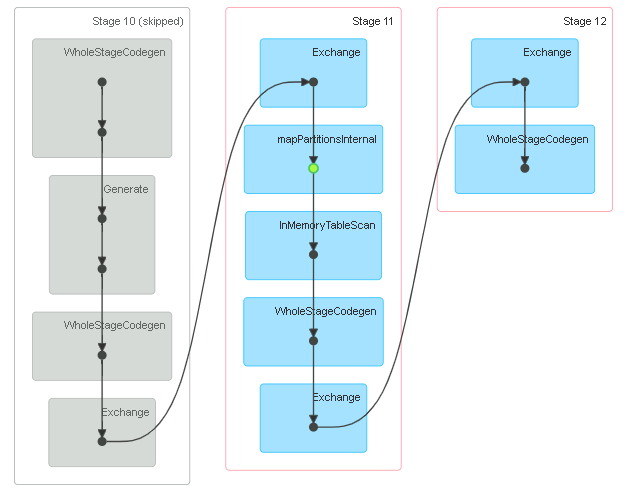
\includegraphics[scale=0.8]{images/3-spark/broad-DAG-3.png}
	\caption{DAG for third job created by Spark when using broadcast on join.}
	\label{fig:spark-broad-DAG-3}
\end{figure}


\section{Performance evaluation}

Performance are evaluated by varying the number of executors and cores per executor. 
Let's consider cluster characteristics (10 nodes, 4 cores per node) and given constraints (usage of 8 CPUs at most).   
Each casuistry result is the average value upon 3 runs. Results are shown in table \ref{table:spark-perf}.

As we can notice, results confirm common best practice rules: best performances among all more promising combinations are obtained using the maximum number of resources (8 CPUs); moreover, the whole application speeds up when assigning more than one core to each executor.

\begin{table}[H]
  \centering
  \begin{tabular}{ |c c|c c c c c| } 
    \hline
    \multicolumn{2}{ |c| }{} & \multicolumn{5}{ c| }{Executors} \\
    \multicolumn{2}{ |c| }{} & 1 & 2 & 3 & 4 & 8 \\
    \hline
    \multirow{3}{4em}{Cores per executor} 
    & 1 &  &    &    &    & 88 \\      
    & 2 &  &    & 94 & 79 & \\ 
    & 3 &  & 96 &    &    & \\     
    \hline
  \end{tabular}
  \caption{Performance results expressed as elapsed time in seconds using \textbf{replication factor = 100} for most promising combinations.}
  \label{table:spark-perf}
\end{table}


